\documentclass{scrreprt}
\usepackage[english]{babel}
\usepackage[euler]{textgreek}
\usepackage{graphicx}
\usepackage{caption}
\usepackage{subcaption}
\graphicspath{ {figures/} }

\begin{document}

% ----------------------------------------------------------------------------
% Titel (erst nach \begin{document}, damit babel bereits voll aktiv ist:
\titlehead{University of Applied Sciences Hamburg}% optional
\subject{Lab report}							% optional
\title{Machine learning}					% obligatorisch
%\subtitle{hi i bims}						% optional
\author{Marc Gehring, 2266937}			% obligatorisch
\date{Dec 2020}								% sinnvoll
\publishers{Prof. Dr. S. Hallerberg}	% optional
\maketitle

% verwendet die zuvor gemachte Angaben zur Gestaltung eines Titels
% ----------------------------------------------------------------------------

% Inhaltsverzeichnis:
\tableofcontents
% ----------------------------------------------------------------------------

% Gliederung und Text:
\chapter{Datasets}
\section{YouTube Trends}
\label{sec:dataset-youtube}
ugö ig igööiug öig ög

\section{MNIST}
\label{sec:dataset-mnist}
The MNIST (Modified National Institute of Standards and Technology) dataset is a set of handwritten digits for training and evaluation of machine learning methods.

dataset of handwirtten digits used for image classification
60k training examples and 10k test examples
each digit is centered and resized to 28x28 pixsels, which makes it suitable for introductory tasks of machine learning
the dataset is said not to be representative benchmark for Computer Vision (CV) tasks anymore

\section{Image Classification Dataset}
\label{sec:image-classification}

\chapter{Machine Learning Methods}
\section{Linear Regression}

\section{Artifical Neural Networks}
An Artifical Neural Network (ANN) is a model to approximate some function y=f*(x). The model f learns the paramters \texttheta to map from x to y. Therefore the model can be described as y = f(x,\texttheta). Usually the model f is represented by chained functions, each of which are called layers of the model. The length of the chain gives the depth of the model.
input output, other layers are hidden layers, conntected by weights
the weights are the transformation from one layer to another and represent the function of each layer.for a single layer it can be written as h = wa+b where b is a bias
to activate a single neuron an activation function is needed, which is usually a nonlinear function
a whole network can be represented as blablabla

with random initialization of the weights the network outputs random values in the last layer. to match the outputs to the labels of the data presented to the network the weights need to be changed. the process of presenting labeled data to the network and changing weights accordingly is called training or learning. A training process consists of two steps known as forward pass and backward propagation. In the forward pass a sample of the training dataset is presented to the network and the output is computed. for this output a quality measure known as the cost function is computed. it maps the difference of the output vector and the label to a scalar value. a simple example is the MSE. to match the output to the labels the cost function is minimized with respect to the parameters. therefore the gradient of the weights with the minimal cost function is computed to update the weights of the network

convolutional layers
conv layers are layers with learnable multidimensional filters instead of scalar weigths between neurons. these filters have a reciptive field like binocluar neurons in the humane visual system. instead of a single value these kernels are producing a two dimensional activation map. during training the network learns to detect special types of features.

\subsection{MNIST Model}
The MNIST dataset introduced in chapter xxx is the hello world of image classification and was a valid benchmark for many years. Due to the already preprocessed and preloaded images there is very little code necessary start with building the model architecture. The model architecture is a simple convolutional network with six hidden layers. The input layer consists of all 784 pixel values which passes the values to the hidden convolutional layers with a subsequent max pooling layer each. The architecture is depicted in \ref{fig:mnist_architecture}. To evaluate the model performance at first the type of activation function is changed and the changes in training and test accuracy are recorded. The activation functions used are as follows.

\begin{itemize}
\item rectified linear unit
\item softmax function
\item sigmoid function
\item hyperbolic tangent function
\end{itemize}

As the second task the model performance in dependency of the model depth shall be evaluated. The activation function is choosen to be a ReLU for all models.

\begin{figure}[h]
\centering
\includegraphics[width=1\textwidth]{mnist_architecture}
\caption{a nice plot}
\label{fig:mnist_architecture}
\end{figure}




\subsection{Image Classification Model}

\section{Variational Autoencoders}


\chapter{Measuring Machine Learning Success}

\chapter{Results}
\section{MNIST Model}
In this section the results of the accuracy study of a simple ConvNet with the MNIST dataset are presented. At first the influence of the acvitation function was evaluated. Four commonly used activation functions were choosen for this task. For the training set the accuracy and the loss function were plotted over seven epochs. It can be seen that the networks with ReL and hyperbolic tangent activation function are performing bettr than the networks with the sigmoid and softmax. The second task adresses the depth of the network and its influence on the test accuracy. For that the number of convolutional layers is increased starting with zero.
\begin{figure}
	\centering
	\begin{subfigure}[H]{0.5\textwidth}
		\includegraphics[width=\textwidth]{mnist_train_performance_activation}
	\end{subfigure}%
	\hfill
	\begin{subfigure}[H]{0.5\textwidth}
		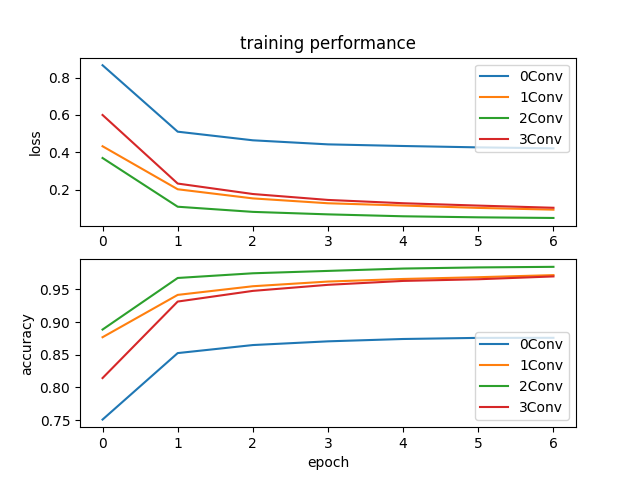
\includegraphics[width=\textwidth]{mnist_train_performance_layers}
	\end{subfigure}
\end{figure}

\chapter{Discussion and Outlook}

\end{document}